\lstnewenvironment{Code}[1][]{\lstset{basicstyle=\small\ttfamily, columns=fullflexible, framexrightmargin=+.1\textwidth, keywordstyle=\color{red}\bfseries, commentstyle=\color{blue},
language=C++, basicstyle=\small,  numberstyle=\tiny, stepnumber=1, numbersep=5pt, frame=shadowbox, #1}}{}

\chapter{Implementazione delle fratture}
Passiamo ora a descrivere le principali classi del codice che definiscono la struttura e le proprietà delle fratture, porgendo particolare attenzione alle classi modificate e a quelle da noi implementate.\\

\begin{figure}[htbp]
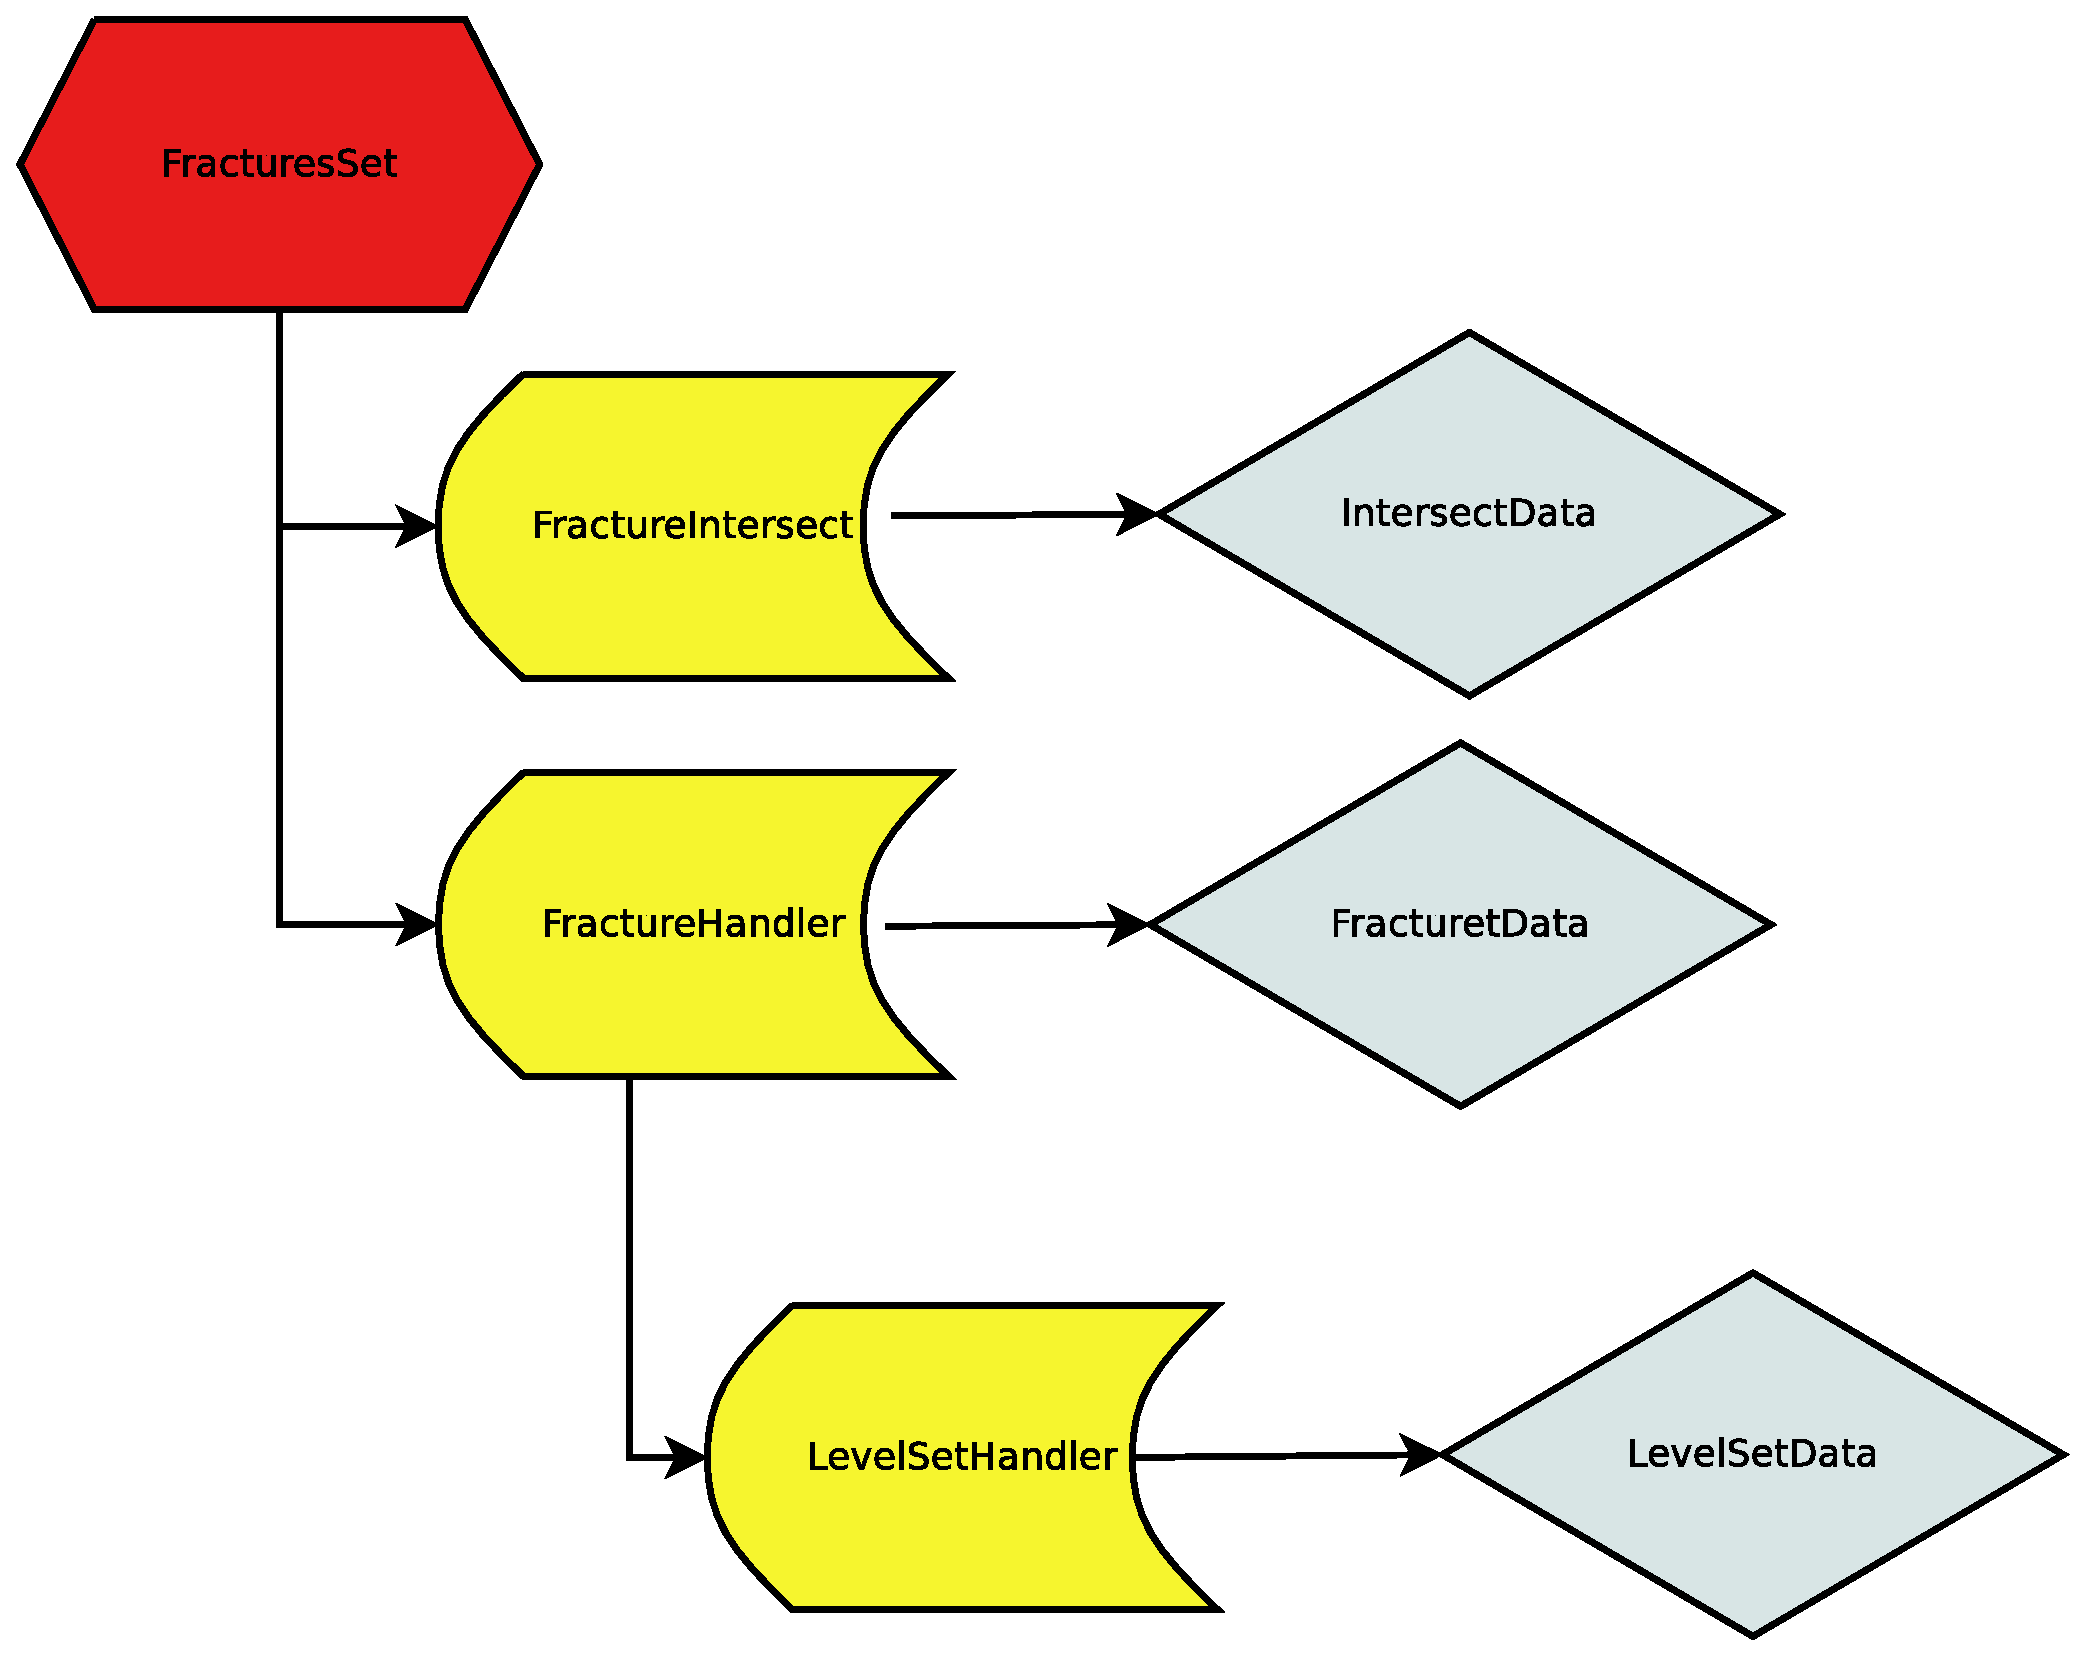
\includegraphics[width=1\textwidth]{img/fratture.eps}
\caption{Inclusione tra le varie classi che costituiscono l'insieme delle fratture}\label{Inclusione classi}
\end{figure}


\par Le classi usate per rappresentare le fratture e le intersezioni si dividono in due categorie:
\begin{enumerate}
\item[-] le classi in cui sono implementati tutti i metodi necessari per la costruzione e la manipolazione della grandezza ( insieme delle fratture, singola frattura, intersezioni, level set). Queste classi sono principalmente denominate col il suffisso \textit{Handler} e costituiscono l'ossatura dell'insieme delle fratture;
\item[-] le classi in cui sono contenuti tutti i parametri geometrici, fisici e le grandezze numeriche per l'implementazione e la risoluzione con elementi finiti, che riguardano la grandezza in esame. Vengono indicate con il suffisso \textit{Data} e rappresentano sempre un campo della corrispondente classe di tipo \textit{Handler}.
\end{enumerate}



\section{La Classe \texttt{FracturesSet}}
La class \texttt{FracturesSet} è la classe che contiente tutte le fratture e le rispettive intersezioni. La funzione che costruisce l'insieme delle fratture e le eventuali intersezioni è la funzione  \texttt{init}, che prende in input tutti i parametri necessari quali il numero di fratture, le mesh per l'integrazione e una variabile di tipo GetPot per la lettura dal file data. 

\begin{Code}[caption={Classe \texttt{FracturesSet}}]
class FracturesSet
{
public:

    enum
    {
        FRACTURE_UNCUT = 10000,
        FRACTURE_INTERSECT = 10000
    };

    FractureHandler ( const GetPot& dataFile,
                      const size_type& ID,
                      const std::string& section = "fractureData/" );

    void init ( );

    [ ... ]

private:
	FracturePtrContainer_Type M_fractures;

	FractureIntersectPtr_Type M_intersections;
	[ .... ]
};
\end{Code}
I campi principali della classe sono:
\begin{enumerate}
\item[-] \texttt{M\_fractures}, variabile di tipo vettore di puntatori alla classe \texttt{FractureHandler}  di cui parleremo più avanti, che rappresenta l'insieme di tutte le fratture;
\item[-] \texttt{M\_intersections}, un puntatore alla classe \texttt{FractureIntersect}, che rappresenta l'insieme di tutte le intersezioni. 
\end{enumerate}


\section{La Classe \texttt{FractureHandler}}

La classe  \texttt{FractureHandler} è la classe che inizializza e gestisce ogni frattura. I principali campi di questa classe sono:
\begin{enumerate}
\item[-] \texttt{M\_data}: classe \texttt{FractureData} che contiene tutte le informazioni circa la natura geometrica e fisica della singola frattura;
\item[-] \texttt{M\_levelSet}: puntatore alla classe \texttt{LevelSetHandler} di cui parleremo più avanti;
\item[-] i metodi di integrazione e le mesh per pressione e velocità;
\item[-] il vettore dei gradi di libertà estesi per velocità e pressione.
\end{enumerate}

La particolarità di questa classe è che possiede due mesh: una mesh 2d \texttt{M\_meshMapped} e una mesh 1d \texttt{M\_meshFlat}. Questo deriva dal fatto che le fratture sono su un piano e hanno una rappresentazione del tipo $y=f(x)$, cioè i loro punti hanno coordinate $(x,y)$. La libreria che noi usiamo, \textit{GetFEM++}, non è in grado di integrare su una mesh i cui punti hanno coordinate $(x,y)$ un'equazione 1d come quella del nostro modello ridotto. La tecnica è quindi quella di risolvere il problema integrando sulle mesh " piatte " 1d ottenute proiettando le mesh reali, e successivamente interpolare i risultati ottenuti per ritornare sulle mesh 2d. La creazione delle mesh è nella funzione \texttt{ init}.
\par La funzione principale di questa classe è  \texttt{setMeshLevelSetFracture }.
Tale funzione crea un legame tra la frattura corrente e le fratture con cui ha un'intersezione, tenendo traccia della mesh e dei valori del level set della frattura corrente nei punti della frattura intersecata. Nel caso di intersezione di tipo \textit{Cross}, dove l'intersezione tra due level set non è detto che avvenga su due punti delle rispettive mesh, vengono aggiunti i gradi di libertà estesi, due per la velocità e uno per la pressione. Nel caso dell'intersezione di tipo \textit{Bifurcation} l'introduzione di tali elementi non si rende necessaria.


\begin{Code}[caption={Funzione \texttt{setMeshLevelSetFracture}}]
size_type FractureHandler::setMeshLevelSetFracture ( 
					FractureHandler& otherFracture,
					size_type& globalIndex,
				         const std::string& type )
{	
[ ... ]
if ( !M_meshLevelSetIntersect[ otherFractureId ].get() )
{
   M_meshLevelSetIntersect[ otherFractureId ].reset
	 ( new GFMeshLevelSet_Type ( M_meshFlat ) );
   LevelSetHandlerPtr_Type otherLevelSet = otherFracture.getLevelSet();
   M_levelSetIntersect [ otherFractureId ].reset 
	( new GFLevelSet_Type ( M_meshFlat, 1, false )  );
   M_levelSetIntersect [ otherFractureId ]->reinit();

   const size_type nbDof = 
	M_levelSetIntersect [ otherFractureId ]->get_mesh_fem().nb_basic_dof();

   for ( size_type d = 0; d < nbDof; ++d )
   {
      base_node node = M_levelSetIntersect [ otherFractureId ]
			->get_mesh_fem().point_of_basic_dof(d);
      base_node mappedNode ( node.size() +1 );
      scalar_type t = d*1./(M_data.getSpatialDiscretization () );
      base_node P (node.size());
      P [0] = t;
      mappedNode [0] = node [0];
      mappedNode [1] = M_levelSet->getData()->y_map ( P );
      M_levelSetIntersect [ otherFractureId ]->values(0)[d] = 
	otherLevelSet->getData()->ylevelSetFunction ( mappedNode );
   }

   M_meshLevelSetIntersect[ otherFractureId ]
	->add_level_set ( *M_levelSetIntersect [ otherFractureId ] );
   M_meshLevelSetIntersect[ otherFractureId ]->adapt ();

   size_type i_cv = 0;
   dal::bit_vector bc_cv =
   M_meshLevelSetIntersect[ otherFractureId ]->linked_mesh().convex_index();
		
   for ( i_cv << bc_cv; i_cv != size_type(-1); i_cv << bc_cv )
   {
     if ( M_meshLevelSetIntersect[ otherFractureId ]->is_convex_cut ( i_cv ) )
     {  
        if ( type == "Cross")
        {	
           M_meshFlat.region ( FractureHandler::FRACTURE_UNCUT 
		* ( M_ID + 1 ) ).sup ( i_cv );
	 M_meshFlat.region ( FractureHandler::FRACTURE_INTERSECT 
		* ( M_ID + 1 ) + otherFractureId + 1 ).add( i_cv );
	 M_extendedPressure.push_back ( 
		M_meshFEMPressure.ind_basic_dof_of_element ( i_cv )[0] );
	 M_extendedVelocity.push_back ( 
		M_meshFEMVelocity.ind_basic_dof_of_element ( i_cv )[0] );
	 M_extendedVelocity.push_back ( 
		M_meshFEMVelocity.ind_basic_dof_of_element ( i_cv )[1] );
        }
            	
       M_fractureIntersectElements [ otherFractureId ].push_back ( i_cv );
	
           [ ... ]
      }
   }
}

return numIntersect;
}
\end{Code}


\section{Le Classi \texttt{LevelSetHandler} e \texttt{LevelSetData}}
Le fratture sono rappresentate come delle rette, funzioni $y=f(x)=ax+c$. Ad ogni frattura è associata una funzione level set  del tipo $f(x,y)=y-ax-b$ che divide il piano in due semipiani: i punti un cui $f(x,y)>0$ e i punti in cui $f(x,y)<0$. I punti in cui $f(x,y)=0$ sono quelli in cui è definita la frattura. 
\par La classe \texttt{LevelSetHandler} inizializza il levelset associato alla frattura. 
La funzione fondamentale della classe è la funzione \texttt{init}, funzione che inizializza il level set, definisce i metodi di integrazione e aggiunge alla mesh di supporto l'informazione legata al level set. I campi fondamentali della classe sono:
\begin{enumerate}
\item[-] \texttt{M\_data}: puntatore alla classe \texttt{LevelSetData}, classe che contiene tutte le informazioni sul level set e le funzioni per valutarne il valore nei punti;
\item[-] \texttt{M\_mesh}: puntatore ad una variabile di tipo \textit{getfem::mesh\_level\_set}, classe che contiene informazioni sulla mesh tagliata da level set;
\item[-] \texttt{M\_levelSet}: oggetto di tipo \textit{getfem::level\_set}, variabile che definisce il level set. In GetFEM un level set è rappresentato come una o due funzioni scalari, definito su una mesh di tipo \textit{getfem::mesh\_fem}, ossia una mesh su cui è definito un metodo ad elementi finiti.
\end{enumerate}

\begin{Code}[caption={Classe \texttt{LevelSetHandler}}]
class LevelSetHandler
{
public:

    LevelSetHandler ( const GetPot& dataFile, 
			const std::string& section =  "fractureData/", 
    			const std::string& sectionLevelSet = "levelSet/" );

    void init ( getfem::mesh& mediumMesh,
		    const std::string& mediumIntegrationTypeVelocity,
		    const getfem::mesh_fem& mediumMeshFEMPressure,
		    const getfem::mesh_fem& mediumMeshFEMVelocity );

	[ ... ]
private:

    LevelSetDataPtr_Type M_data;

    GFMeshLevelSetPtr_Type M_mesh;

    GFLevelSetPtr_Type M_levelSet;
	[ ... ]
};
\end{Code}


 \section{Le Classi \texttt{FractureIntersect} e \texttt{IntersectData}}

La classe \texttt{FractureIntersect} rappresenta tutte le intersezioni tra le fratture. Ad ogni tipo di intersezione viene associato il vettore delle classi \texttt{IntersectData}, classe che rappresenta la vera e propria intersezione, tenendo traccia delle informazioni sulle fratture e dell'id dell'elemento della mesh di supporto in cui avviene l'incontro.
\par Le intersezioni vengono classificate come \textit{Parallel}, \textit{Cross} e \textit{Bifurcation}.  L'idea alla base della classificazione è quella di considerare gli elementi della mesh 2d di supporto, la mesh del mezzo, in cui passano due o più fratture, e di associargli un flag:
\begin{enumerate}
\item[-] \textit{Parallel}: quando due o più fratture passano in uno stesso elemento della mesh ma non si intersecano;
\item[-] \textit{Cross}: quando due fratture passano nello stesso elemento della mesh e si intersecano formando una \textit{X};
\item[-] \textit{Bifurcation}: quando tre fratture si intersecano in un punto comune formando una \textit{Y}.
\end{enumerate}

\begin{Code}[caption={Funzione \texttt{constructIntesection}}]
void FractureIntersect::constructIntesection ( 
	const getfem::mesh& mesh, getfem::mesh_level_set& meshLevelSet, 
	const FracturePtrContainer_Type& fractures )
{
[ ... ]
meshLevelSet.find_level_set_potential_intersections ( 
			listOfConvex, listOfLevelSet_bitVector );

sizeVectorContainer_Type listOfLevelSet ( listOfConvex.size() );

if( listOfConvex.size() > 0 )
{
   for ( size_type i = 0 ; i < listOfConvex.size(); ++i )
   {
      // Conversione da un vettore di bit a un vettore di interi
      fromBitVectorToStdVector ( 
      listOfLevelSet_bitVector [ i ], listOfLevelSet [ i ] );

       // Per ogni elemento della mesh di supporto in cui passano 
      // almeno due fratture verifico il tipo di intersezione
       IntersectionType type = intersectionType ( 
		meshLevelSet, listOfConvex [ i ], listOfLevelSet [ i ] );
	        
       // Prendo i puntatori alle fratture coinvolte
      FracturePtrContainer_Type fracturesInvolved ( listOfLevelSet[i].size() );

      for ( size_type f = 0; f < fracturesInvolved.size(); ++f )
      {
	 fracturesInvolved [ f ] = fractures [ listOfLevelSet [ i ] [ f ] ];
       }
       // Costruisco la classe IntersectData per la nuova intersezione 
       // e la aggiungo in base al tipo
      IntersectData intersection;
      intersection.setIntersection ( listOfConvex[i], fracturesInvolved );		
      M_intersections [ type ].push_back ( intersection );
    }
[ ... ]
}

\end{Code}

\par La funzione  \texttt{constructIntesection} contiene la classificazione delle intersezioni. In questa funzione viene data una numerazione globale alle intersezioni, prima quelle di tipo \textit{Cross} e poi quelle di tipo  \textit{Bifurcation}.  Nel caso delle prime vengono aggiunte due nuove incognite, una per ogni frattura, necessarie per imporre le condizioni d'interfaccia nella formulazione debole del problema. Queste nuove variabili rappresentano la pressione nel punto di intersezione e  vengono poi accoppiate in modo da risultare uguali. Nel secondo caso invece si introduce una sola incognita per ogni intersezione, variabile che rappresenta la pressione nel punto d'incontro. Per ogni frattura coinvolta inoltre si tiene traccia del grado di libertà in cui avviene l'intersezione. Questo perchè, come vedremo, la condizione al contorno deve essere imposta solo del grado di libertà dell'estremo libero della frattura.